%**************** SoTA **************

\chapter{State of the Art}
\label{chapter:sota}
As presented in the introductory chapter, this dissertation focuses on two main applications: automatic transcription and spoken language translation. In the first part of this chapter, I will give an overview on the main research areas that are related to these two topics with a focus on neural network based approaches. Automatic transcription, which is made possible with \textit{automatic speech recognition (ASR)}, is explained in Section \ref{sota:asr}. Approaches to the problem of punctuation recovery in ASR output are presented in Section \ref{sota:punk_on_asr}. \textit{Neural machine translation} is presented in Section \ref{sota:nmt} with a focus on \textit{spoken language machine translation}. After a brief introduction to text-to-speech synthesis (TTS) systems in Section \ref{sota:tts}, I will present the concept of speech-to-speech translation with recent work on its field in Section \ref{sota:s2s}.

The second part of this chapter reviews relevant work on the inclusion of prosody into these systems. Focus is given on usage of prosody in punctuation recovery in Section \ref{sota:punk_prosody} and adding prosodic modalities on spoken language translation in Section \ref{sota:prosody_in_smt}. 

\section{Neural Speech Processing Overview}
%speech processing systems overview

A speech processing system consists of at least one of the following modules: Automatic Speech Recognition (ASR) for converting verbal communication into discrete symbolic form (i.e.~text), text-to-speech (TTS) system for generating information in spoken form, and a spoken language understanding (SLU) system for mapping between actions and verbal utterances \citep{slp_book}. Depending on the application, versions and combinations of these systems are employed to solve the task involved with it. For instance, an automatic subtitling system would involve an ASR system together with a speech activity detection module to transcribe the spoken parts in a media. If the subtitling is to be done in another language, the same pipeline would be followed by a machine translation system. A complete speech-to-speech pipeline would result in an automatic dubbing system where translated content would be synthesized using a TTS system. 

%neural networks overview. 
Research on these subareas of speech technology has recently experienced a great shift towards the usage of \textit{artificial neural networks (ANN)}. Popularity of ANN in general has risen in the recent years mostly due to advancements in computing power. Specifically, training of large and deep neural networks in a reasonable amount of time has been made possible with \textit{Graphical Processing Units (GPUs)}.  

I will introduce briefly the concept of \textit{deep neural networks (DNNs)} as they form the basis of the experimentation presented in this dissertation. The information presented in this section can be consulted in \cite{shigeru2000handbook} and \cite{bengio_dl} for a deeper understanding. 

\subsection{Deep Neural Networks}
\label{sota:dnns}

\begin{figure}[t]
  \centering
  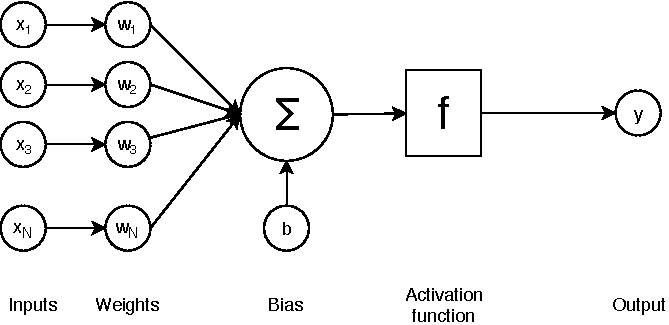
\includegraphics[width=0.6\linewidth]{img/perceptron.pdf}
  \caption{An artificial neuron.}
  \label{sota:neuron}
\end{figure}

An artificial neural network consists of a group of nodes that are modeled after the neurons in a biological neural system and connections between them modelling the axons in the neural system. Figure \ref{sota:neuron} illustrates the structure of one neural node, which is also referred as \textit{perceptron} or simply \textit{neuron}. Each connection towards a neuron is an input ($x_i$) and is associated with a weight coefficient ($w_i$). The basic function of a neuron defines the input signal to the neuron as:
\begin{equation}
    a = \sum _{ i }{ w_i x_i + b} 
\end{equation}

The input signal is then passed into an activation function to produce the output $y$. 

\begin{equation}
    y = f(a)
\end{equation}

Activation function is a differentiable function that resembles a step function so the neuron \textit{fires} with certain input. The original Rosenblatt's perceptron had Heaviside step function as the activation function \citep{Rosenblatt58theperceptron}. Activation functions commonly being used today are the \textit{sigmoid} and the \textit{hyperbolic tangent} functions. 

One single neuron is evidently not sufficient for modelling complex functions. A basic neural network consists of a layer of input neurons fully connected to a layer of output neurons. This setting produces an N-to-M mapping. Extra layers are added between the input and output layers to introduce even more complexity to the network. These layers are called \textit{hidden layers} and are fully connected between each other between input and output layers. An illustration of a neural network with two hidden layers is given in Figure \ref{sota:neuralnet}. Number of hidden layers can be determined according to the task-at-hand. A neural network with more than one hidden layer is called a \textit{deep neural network} \citep{yoav}. 

\begin{figure}[t]
  \centering
  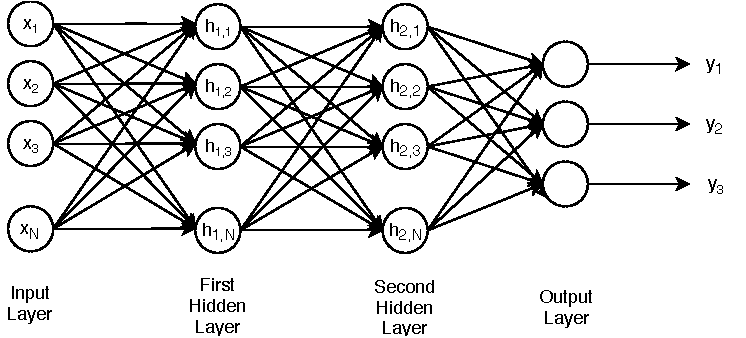
\includegraphics[width=0.9\linewidth]{img/NeuralNet.pdf}
  \caption{A fully connected feed-forward neural network with two hidden layers.}
  \label{sota:neuralnet}
\end{figure}

Although there exist many types of neural network taxonomies, one important characteristic that divides neural network architectures into two is the direction of the signal flow in the network. A \textit{feed-forward} architecture (as in the example in Figure \ref{sota:neuralnet}) allows information to be passed in only one direction. Whereas a \textit{recurrent neural network (RNN)} architecture allows the output signal of some nodes to be passed again to a neuron coming previously, or to the neuron itself. Recurrent neural networks are especially suitable for representing time-series data. Because of this, it is currently being preferred as the principal architecture on many state-of-the-art applications of machine translation, speech recognition and speech synthesis. 

\begin{figure}[t]
  \centering
  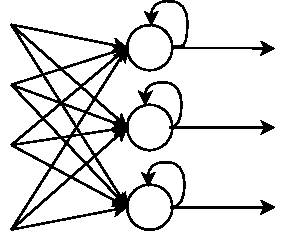
\includegraphics[width=0.3\linewidth]{img/RecurrentNeuralNet.pdf}
  \caption{Information flow in a recurrent neural network (RNN). Output signals are allowed to go back as input signals to the neurons. }
  \label{sota:rnn}
\end{figure}

As it can be seen in Figure \ref{sota:rnn}, a neuron in a RNN can have its output connected back to itself as an input. This model allows the neuron to keep a form of a \textit{memory} from previous inputs and decide on the next output according to it together with the current input. Another advantage the RNN architecture gives is the ability to represent different mappings between nodes at each time step. Figure \ref{sota:rnn_connections} shows types of connections between \textit{RNN cells}, which can be one-to-one, one-to-many, many-to-one or many-to-many. An application to a many-to-many network would be translation, where a sequence of words are encoded and then decoded in another language. An example of a many-to-one network would be e.g. voice classification given an acoustic feature sequence. This group of neural networks are sometimes called \textit{encoder-decoder networks}. Many-to-many type RNN is sometimes referred as \textit{sequence-to-sequence network}. 

\begin{figure}[t]
  \centering
  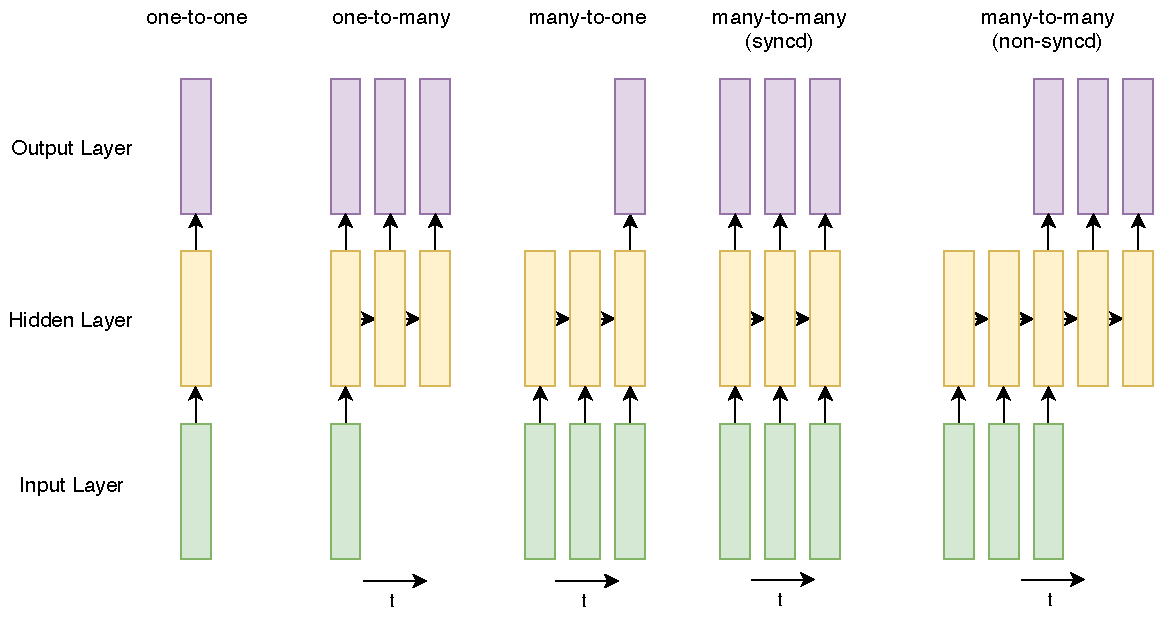
\includegraphics[width=0.8\linewidth]{img/rnn_types.pdf}
  \caption{Four types of RNNs in terms of input and output type. }
  \label{sota:rnn_connections}
\end{figure}

%backpropagation
Neural network training involves the following steps: Introduction of samples in the training set to the network, computing the error with help of a \textit{loss function} comparing desired output to the networks output, computing the gradient given by the error and then shifting the network weights in the direction and magnitude of the gradient. One common method used in performing this operation is \textit{stochastic gradient descent (SGD)} \citep{bengio_dl, sgd2}. 

Although the aim of training is to minimize the total loss given by all training samples, optimization is performed at introduction of each sample. To avoid unnecessary amount of fluctuations (i.e.~noise) in weight updates, samples are generally inputted in batches, an average loss is calculated and then network is updated according to that average loss.  

A key step in training is the step where gradients are calculated according to the loss that the network gives. This is performed through a method called \textit{backpropagation algorithm}, which is the process of going backwards through the network calculating the partial derivative of the error at each weight \citep{Rumelhart:1988:LRB:65669.104451}. These derivatives are then used to update the weights using a method called \textit{gradient descent}. This update is scaled by the \textit{learning rate}, which is a pre-determined \textit{hyperparameter} that is sometimes allowed to decay in time to enable fine-tuning of the network during later steps of the training. 

%TODO: vanishing, exploding gradient and overfitting will come here
% overfitting is addressed with regularization. From \cite{Klejch}:We addressed this problem using a regularization approach based on dropout \cite{JMLR:v15:srivastava14a}, which forces a neural network to learn a more robust representation by randomly resetting a portion of activations of nodes during training.

%\textit{long short-term memory (LSTM)}  \citep{lstm}  %(https://towardsdatascience.com/recurrent-neural-networks-and-lstm-4b601dd822a5)

%TODO: GRU
%Gated recurrent units (GRU), was introduced as a simpler variant of LSTM units , GRUs make computation simpler by having fewer parameters. Number of gates in hidden units are reduced to two: (a) the \textit{reset} gate determines whether the previous memory will be ignored, and (b) the \textit{update} gate determines how much of the previous memory will be carried on. 

%GRU figure

\subsection{Automatic Speech Recognition}
\label{sota:asr}

In its most simple sense, automatic speech recognition (ASR) is the conversion of speech in its acoustic form into a symbolic form such as words or letters. It is the probabilistic modelling of the question "What is the most probable word sequence among all possible word sequences given an acoustic input?". Figure \ref{sota:asr_process} illustrates this process. Speech signal captured by microphone is first encoded into a sequence of acoustic feature vectors. Following, the acoustic feature vectors are decoded into the words that represent the linguistic information that lies in the speech signal. 

\begin{figure}[t]
  \centering
  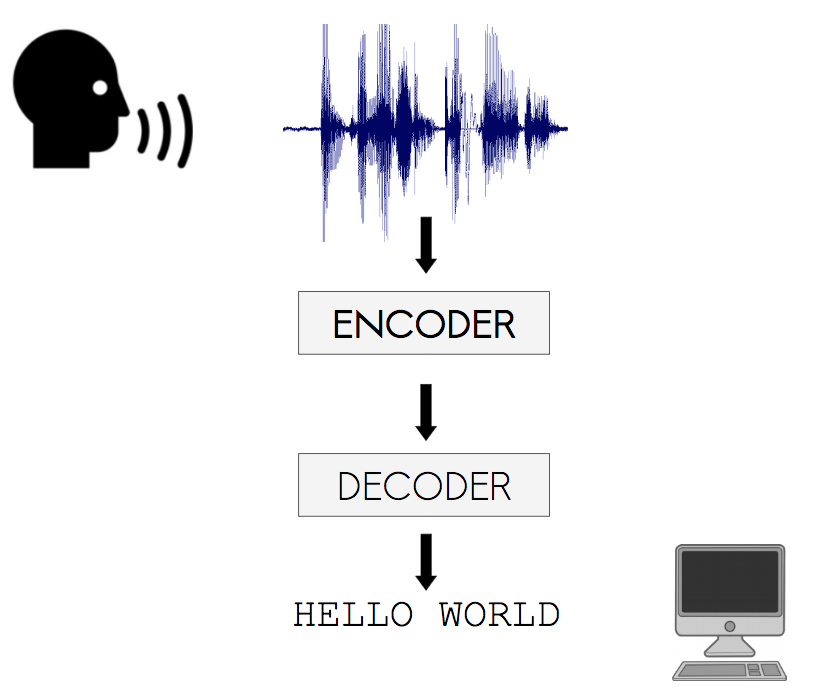
\includegraphics[width=0.7\linewidth]{img/asr_schema.png}
  \caption{Speech recognition is the conversion of an acoustic signal with spoken language into its written form. }
  \label{sota:asr_process}
\end{figure}

Classical approaches to ASR employ a modeling of spoken language that uses Gaussian mixture model-hidden Markov model (GMM-HMM). HMM is a powerful statistical method for representing time-series data \citep{slp_book, hmm_balls}. A GMM-HMM ASR system has a modular architecture: The feature extraction step converts the input speech signal into a sequence of fixed size acoustic vectors. Later, the decoder makes use of the acoustic model, the language model and the pronunciation dictionary in order to decide the most likely word sequences they represent. Acoustic and language models are trained with a corpus of transcribed speech samples and a text corpus. While the acoustic model stores the information of the statistical behaviour of the sounds in a language, the language model stores the likelihood of the tokens (words) occurring and co-occurring in a language. 

\begin{figure}[t]
  \centering
  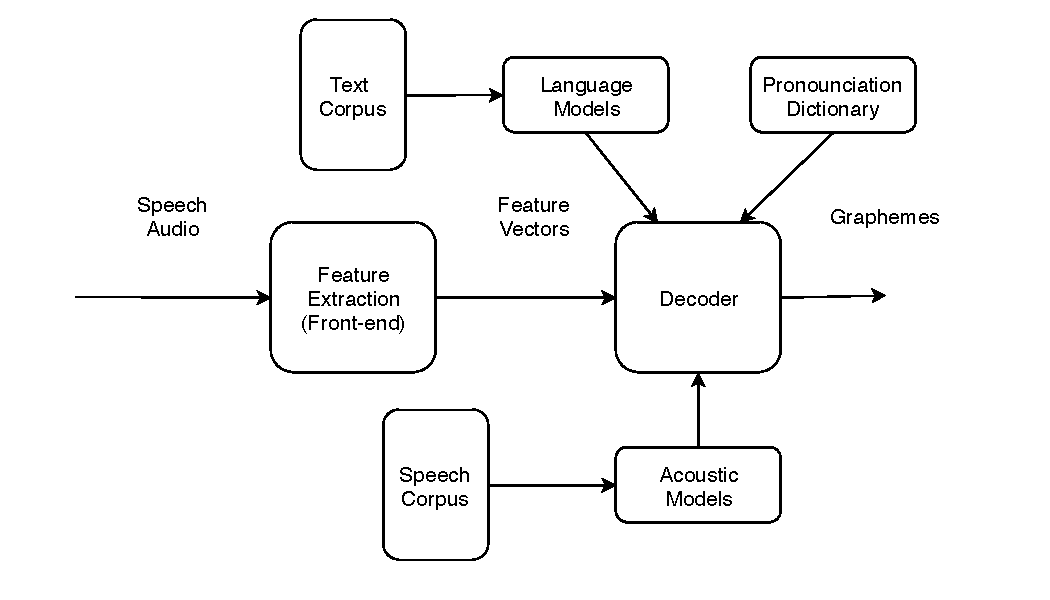
\includegraphics[width=0.8\linewidth]{img/asr2.pdf}
  \caption{General architecture of a traditional ASR system.}
  \label{sota:asr_schema}
\end{figure}

ASR systems experienced a breakthrough with the use of deep neural networks from 2012 on with its introduction in \cite{asr_dnnhmm}. The DNN-HMM ASR replaced the feature representation step that used Gaussian mixtures with a recurrent neural network architecture. This configuration replaced the modular architecture that separated language and acoustic models in the traditional setup and thus minimized the complexity of the system. The graphical comparison of two models is illustrated in Figure \ref{sota:gmm-dnn-hmm}. The DNN-HMM based ASR showed an improvement of 20\% compared to the GMM-HMM based. 

\begin{figure}
\begin{tabular}{cc}
  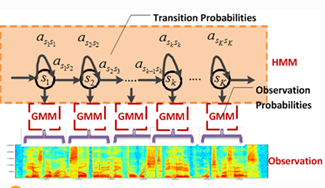
\includegraphics[width=0.5\linewidth]{img/gmm-hmm.png} &   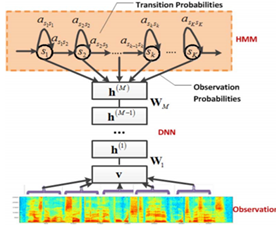
\includegraphics[width=0.5\linewidth]{img/dnn-hmm.png} \\
(a) GMM-HMM & (b) DNN-HMM\\[6pt]
\end{tabular}
\caption{Comparison between GMM based (a) and DNN based (b) ASR (Figure from \cite{asr_dnnhmm})}
\label{sota:gmm-dnn-hmm}
\end{figure}

\subsection{Punctuation Restoration in ASR}
\label{sota:punk_on_asr}

As applications of automatic speech recognition vary greatly, the objective of ASR is only focused on the recognition rate of the words. Aspects such as capitalization and punctuation, which are crucial elements for readability of the ASR output, is generally considered apart from an ASR system. For example, for applications such as automatic captioning or transcript extraction, punctuation and capitalization prove to be essential for improving readability. \cite{Tundik2018} evaluate the effect of presence of punctuation in captions from a end-user perspective and show that punctuated captions are easier to read both when transcriptions are manually or automatically generated. Another case where punctuation proves to be essential is when subsequent processing steps in a pipeline are optimized to work with it. Syntactic or semantic parsing, which is an important module in dialog based systems necessitates input segmented into sentence-like units to function. Most machine translation systems are trained with single sentence input. Furthermore, it is proved that both of these processes function better with properly placed in-sentence punctuation and especially commas \citep{10045_76089, Jones:1994:ERP:991886.991960}. 

%from CSL
% TEXT
The problem of punctuation restoration has been addressed in several works in the literature ---as has been the closely-related issue of boundary detection. Both problems have been tackled from diverse perspectives. In terms of which types of features are used, the approaches fall into three categories: (1) models based only on only textual (lexical and syntactic) features, (2) models based only on only prosodic/acoustic features and finally (3) models where both textual and acoustic/prosodic features are used. In this section I will focus on models based only on textual features. That is, as illustrated in Figure \ref{sota:figure:punc_on_text}, punctuation process is only applied on the raw ASR output without any other cues. 

\begin{figure}[t]
  \centering
  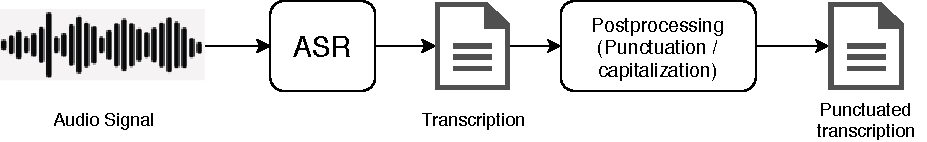
\includegraphics[width=\linewidth]{img/Punctuation_on_ASR_output.pdf}
  \caption{Punctuation and capitalization as a postprocessing step after ASR.}
  \label{sota:figure:punc_on_text}
\end{figure}

Punctuation using only textual features is relevant when e.g.~punctuation restoration is needed for written data \citep{jakubicek2010punctuation} or in the case when corresponding audio information is lost \citep{lu2010better}. In \cite{jakubicek2010punctuation}, for instance, the punctuation detection is addressed from a syntax-based perspective by using the output of an adapted chart parser, which provides information on the expected punctuation placement. In \cite{ueffing2013improved}, several textual features including language model scores, token n-grams, sentence length and syntactic information extracted from parse trees are combined using conditional random fields (CRF). They demonstrate that syntactic features help only when the input language is well-structured (as e.g. newspaper texts). In \cite{lu2010better}, the task is based on dynamic conditional random fields and applied to a conversational speech domain where sentence boundaries and types are detected. 

Another reason that facilitates the usage of solely textual features is the abundance of well-punctuated written data. Using a purely text-based n-gram language model, \cite{Gravano} demonstrate the performance improvement induced by large textual training in punctuation detection and capitalization. Although narrow-range grammatical constructions are recognized well for comma and period placement, n-gram approach fails in discovering long-range dependencies for the correct placement of question marks. 

%TODO: Take the prosodic stuff out 
Punctuation placement is also approached as a monolingual machine translation problem in \cite{peitz2011modeling, Cho2017NMTbasedSA, Paulik} where target sequence is the punctuated version of the source sequence. Also, in \cite{Klejch}, frame-level prosodic features (only pitch and pause) are integrated in a neural machine translation based system with a hierarchical encoder.  

Recently, recurrent neural networks are shown to be suitable for punctuation restoration for their ability to capture long-range dependencies in sequential data. \cite{ballesterosneural} introduce a language-independent model with a transition-based algorithm using LSTMs \citep{lstm}, without any additional syntactic features. \cite{Treviso} experimented with different word embeddings model within an RNN setting and proves that a good word embeddings model improves punctuation restoration accuracy. 

\subsection{Neural machine translation}
\label{sota:nmt}

Machine Translation is defined as the automatic conversion of a sequence of symbols in one language to a sequence of symbols in another language \citep{bengio_dl}. It has evolved through years from rule-based systems (RBMT) to statistical approaches (SMT), which modeled the probabilities of mappings between sub-phrases of various sizes. These probabilities are learned in a statistical fashion from \textit{parallel texts} where sentence aligned translations are available in the languages involved (referred as source and target languages). 

Neural machine translation (NMT) quickly replaced SMT in the recent years for its relatively simpler architecture. It no longer needed fine-tuning of smaller components involved in a SMT system and directly learned mapping from input text sequence to the target text sequence \citep{bahdanau, google_nmt}.

\begin{figure}[t]
  \centering
  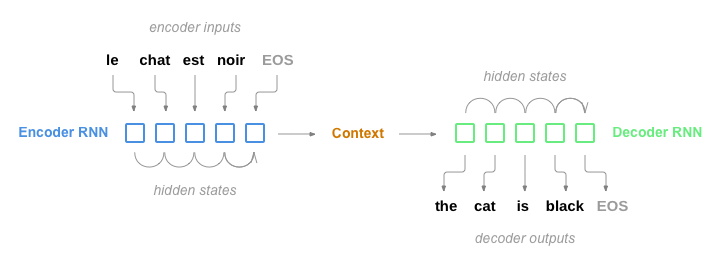
\includegraphics[width=\linewidth]{img/spro_nmt.png}
  \caption{Architecture of an encoder-decoder neural machine translation system. (Diagram taken from \textit{spro}'s sequence-to-sequence translation tutorial on github\footnote{\url{https://github.com/spro/practical-pytorch/blob/master/seq2seq-translation/seq2seq-translation-batched.ipynb}})}
  \label{sota:nmt_schema}
\end{figure}

\begin{figure}[t]
  \centering
  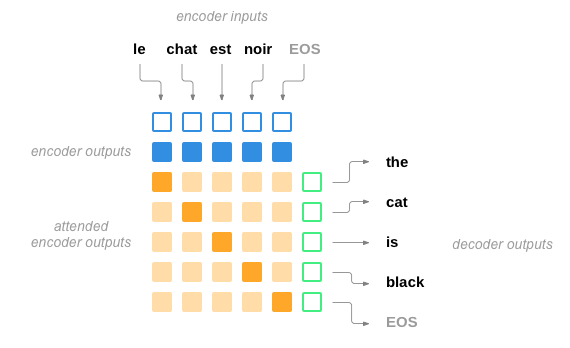
\includegraphics[width=0.8\linewidth]{img/spro_nmt_attention.png}
  \caption{Attention mechanism in encoder-decoder NMT architecture keeps track of portions of the input sequence that affects each decoder output. (Diagram taken from \textit{spro}'s sequence-to-sequence translation tutorial on github\footnote{\url{https://github.com/spro/practical-pytorch/blob/master/seq2seq-translation/seq2seq-translation-batched.ipynb}})}
  \label{sota:nmt_attention}
\end{figure}

A commonly used architecture for NMT is the encoder-decoder architecture, which was introduced earlier in this section\footnote{There exist more types of neural architectures for machine translation task such as the \textit{Transformer}. They are not reviewed in this section as they are not used in this dissertation. }. As illustrated in Figure \ref{sota:nmt_schema}, token sequence in the source language input through an encoder is sent over a decoder to output tokens of the target language. Similar to the data-driven approach of SMT, this network is trained with parallel text to maximize the probability of a correct translation given a source sentence \citep{bahdanau}.

One weakness that this model introduces is the connection between two RNNs that squeezes the input sequence into one single-length vector before being decoded as target token sequence. This is analogous to reading a phrase from beginning to end and then translating it into another language without looking at it again. Normally, a translator would break a input sentence into smaller portions and translate step by step giving attention to a different parts each time. An analogy of this approach was implemented in NMT with the introduction of \textit{attention mechanism} \citep{bahdanau, luong}. As illustrated in Figure \ref{sota:nmt_attention}, the attention mechanism helps focus on different parts of the input at each step of decoding. This relieves the decoder from having to predict target language tokens in one go without any spacial context of the input phrase \citep{google_nmt}. 

\textbf{Spoken language machine translation} is a type of MT where input and/or output to the system is spoken language. Spoken input translation can be employed through the usage of ASR prior to MT and translation can be generated as speech with a TTS to obtain spoken output. Machine translation with spoken input introduces its own specific challenges. For example, written and spoken language show linguistic differences thus models trained on one domain do not necessarily serve to be optimal in the other domain. 

\begin{figure}[t]
  \centering
  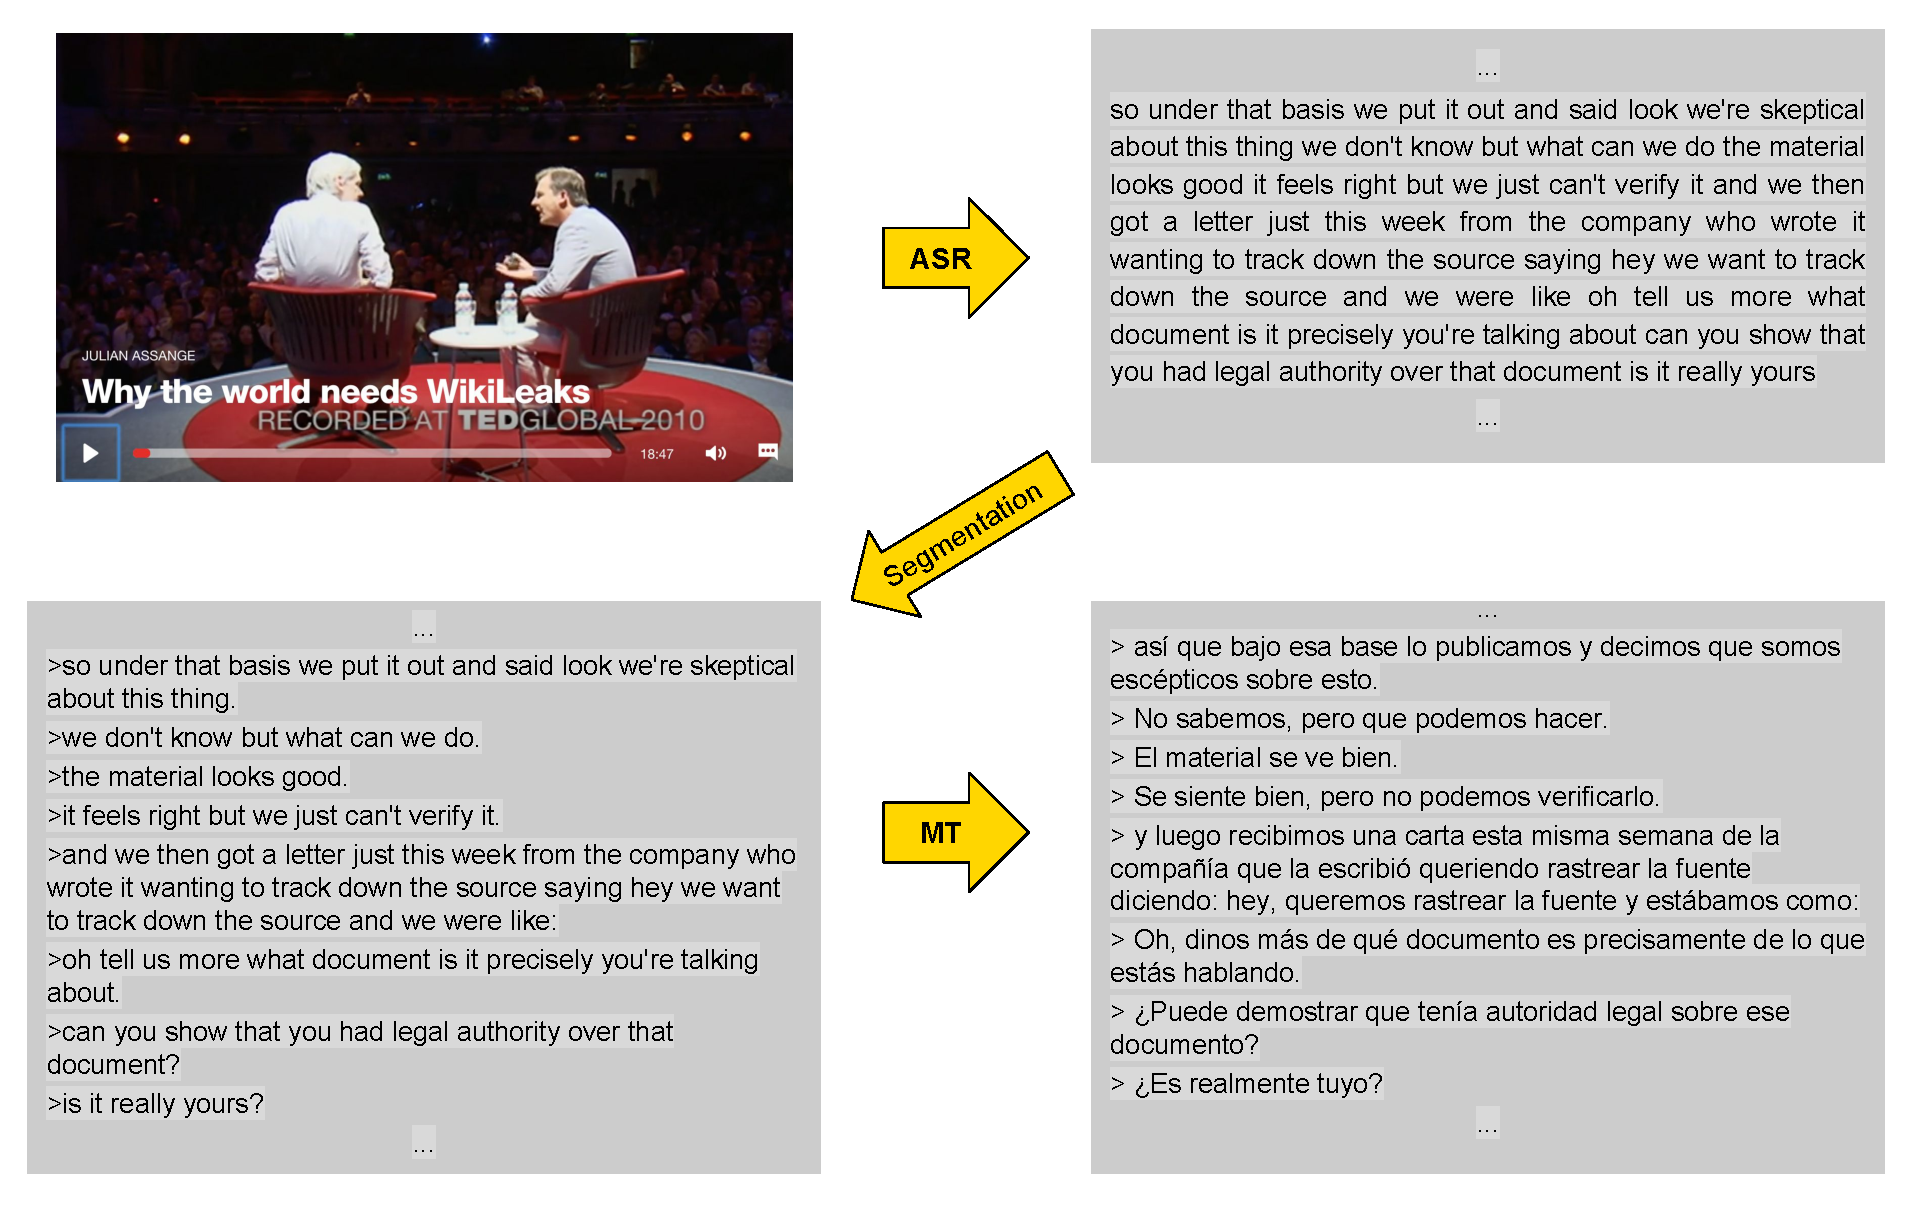
\includegraphics[width=\linewidth]{img/slmt_on_ted.pdf}
  \caption{Spoken language translation demonstrated on a conference recording.}
  \label{sota:tv_transcription}
\end{figure}

One challenge that spoken language translation introduces is the possible incompatibility between ASR output structure and MT input structure. MT models are usually trained with sentence-like structures as samples and therefore show low performance on partial sentence or long sequences of words as input. In text translation domain, processing of long text documents is performed by translating it sentence by sentence using punctuation information as segmentation cues. A similar approach needs to be followed when input is spoken utterances as well. Figure \ref{sota:tv_transcription} \mireia{TODO[this figure is two pages later: too far from text]} illustrates an example of spoken language translation of a conference talk. A standard MT system would be unable to translate the unsegmented transcription of the talk. Translation is made possible only through a segmentation process, such as boundary detection or punctuation restoration. 

Another characteristic involved in spoken language translation is the loss of prosodic information in the transcription step of a classic spoken language translation system pipeline. Prosodic features that would normally give cues for target translations e.g.~through resolving ambiguity or phrasing are left out. 

%Evaluation metric BLEU could be explained here.

\subsection{Text-to-speech synthesis}
\label{sota:tts}

%TODO: \mireia{[This description does not reflect well the main characteristics of each approach. It seems that statistical one is always better and it is not. Concatenative is of higher quality, although sometimes lacks naturalness and its less flexible. Parametric is of lower quality, not necessarily more natural that the concatenative one, but it is way more flexible. Try to expand a little bit more the two approaches. They both have been very important in the last decades.]}

Speech synthesis involves production of a human-like speech given a text input with computational methods. Before the advent of deep learning, there were two main approaches to text-to-speech (TTS) synthesis: concatenative TTS, and parametric TTS. Concatenative TTS is based on the technique of combining short audio clips together to synthesize the desired text. It is a highly complicated process building concatenative TTS systems and its results generally lack naturalness. In contrast, parametric TTS relies on statistical methods by generating speech with a combination of parameters like F0 and energy. Figure \ref{sota:figure:tts} illustrates the workflow of a parametric TTS system. First, morphemes in the input text are converted to phonemes through a linguistic analysis. Next, features like cepstra, F0, duration, break are calculated to be fed into the \textit{vocoder}. The vocoder finally generates the waveform using these parameters.

%TODO: \mireia{Parametric system? Explain it in the caption. Also: why "linguistic" is lowercased and "Feature" and "Vocoder" are capitalised?}
\begin{figure}[t]
  \centering
  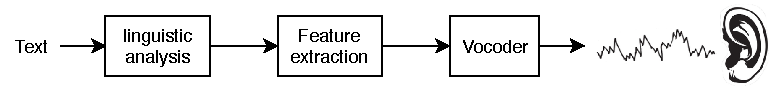
\includegraphics[width=0.9\linewidth]{img/tts_diagram.pdf}
  \caption{Basic workflow of a text-to-speech system.}
  \label{sota:figure:tts}
\end{figure}

What makes relevant TTS in this dissertation is that the Vocoders can take additional parameters in some cases to generate samples with desired features. This is particularly useful in speech-to-speech translation applications where transfer of input prosodic cues to the synthesized target speech is desired. State-of-the-art TTS applications such as \textit{IBM Watson TTS}\footnote{\url{https://text-to-speech-demo.ng.bluemix.net/}} allow this kind of additional parameters to be input in form of \textit{SSML tags}. An example of an input text to a Spanish TTS system with additional prosodic conditioning is shown below: 

%TODO: \mireia{briefly describe which prosodic ssml tags are being used in this example for a non-expert reader.}
\begin{lstlisting}
<p><s>Consciente de su patrimonio espiritual y moral<break time="300ms"/>, la Unión está fundada sobre los valores indivisibles y universales de la dignidad humana, <prosody rate="-15%"> la libertad, la igualdad y la solidaridad, </prosody> y se basa en los principios de la democracia y el Estado de Derecho<break time="500ms"/>.</s> <s><prosody rate="+20%">Al instituir la ciudadanía de la Unión </prosody> y crear un espacio de libertad, seguridad y justicia, sitúa a la persona en el centro de su actuación.</s></p>
\end{lstlisting}

\subsection{Speech-to-speech translation}
\label{sota:s2s}

\begin{figure}[t]
  \centering
  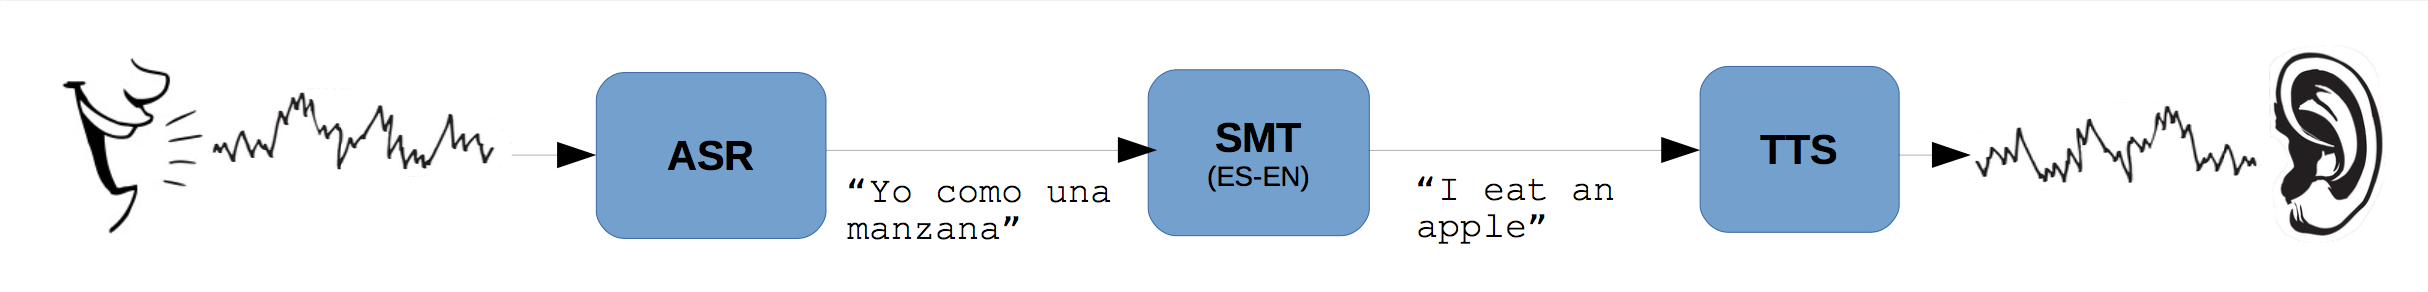
\includegraphics[width=\linewidth]{img/s2s_classic_pipeline.png}
  \caption{A conventional speech-to-speech translation pipeline.}
  \label{sota:s2s_classic}
\end{figure}

Speech-to-speech translation enables human-to-human communication where each of the agents involved speaks in a different language. A device capable of enabling such a communication is able to accept spoken input in language A, translate it to language B and then synthesize it for hearing. By performing this process in both ways, it acts as an interface for a turn-based inter-lingual communication. Conceptually, such a system is the concatenation of the three following processes: (1) Automatic speech recognition, (2) machine translation, and (3) text-to-speech synthesis. A diagram of the one-way process in S2S translation is illustrated in Figure \ref{sota:s2s_classic}. 

There exist various examples of S2S translation solutions resulting from both academic and commercial research. \textit{Verbmobil} is considered as the pioneer in the field as it is the oldest and most extensive research project dealing with S2S translation \citep{wahlster2013verbmobil}. It was designed for translation of spontaneous dialogues in mobile situations for the languages English, German and Japanese. \textit{IBM MASTOR} was developed in a defense oriented framework for facilitating spoken communication in low-resource languages \citep{ibm_mastor}. \textit{TECNOPARLA} was developed with the motivation of spoken translation in the broadcast radio and television domain for the languages Catalan, English and Spanish \citep{tecnoparla}. \textit{EMIME} project was the first work that aimed voice personalization through S2S translation, where synthesized voice is adapted to sound like the recognized voice \citep{emimeemime}. Two projects with Swiss origin, SP2 SCOPES \citep{sp2} and SIWIS \citep{Garner:199815} that focus on Swiss and Eastern European languages report cross-lingual prosodic transfer as their main objectives. Although parallel speech corpora has been published from these projects, there are no recorded results on the accomplishment of these objectives. 

\subsubsection{Spoken parallel corpora}

%TODO: \mireia{I think putting the language acronyms in lowercase will be clearer: en/it/es}

\begin{table*}[ht]
\begin{center}
\begin{tabular}{|l||l|l|l|}
\hline \bf Corpus & \bf Languages & \bf Speech style \\ \hline
EPIC                                            & EN/IT/ES              & spontaneous/interpreted   \\
MSLT                                            & EN/FR/DE              & constrained conversations \\
EMIME                                           & FI/EN, DE/EN          & prompted                  \\
EMIME Mandarin                                  & ZH/EN                 & prompted                  \\
SP2-Speech-Corpus                               & EN/FR/DE/HU/MK/SR     & prompted with emphasis    \\
Japanese-English emphasis                       & JA/EN                 & prompted with emphasis    \\
SIWIS database                                  & EN/FR/DE/IT           & prompted with emphasis    \\
MDA~\citep{almeman2013multi}                    & Four Arabic dialects  & prompted                  \\
Farsi-English~\citep{Melvin2004CreationOA}      & FA/EN                 & read/semi-spontaneous     \\
\hline
\end{tabular}
\end{center}
\caption{\label{sota:corpora} A selection of available parallel speech corpora for use in S2S translation. }
\end{table*}

%Why spoken parallel corpora needed intro
The availability of large parallel corpora is one of the major challenges in developing machine translation systems. Bilingual corpora, which are needed to train statistical translation models, are harder to acquire than monolingual corpora since they presuppose the implication of labour in translation or interpretation. Working on the speech domain introduces even more difficulties since interpretations are not sufficient to capture the paralinguistic aspects of speech. Several attempts have been made to compile large spoken parallel corpora. Some of these corpora published in literature are listed in Table~\ref{sota:corpora}. All of them have been manually compiled in laboratory conditions but show some differences in certain aspects. The EPIC corpus has been compiled from speeches from the European Parliament and their interpretations \citep{bendazzoli2005approach}. The EMIME database is a compilation of prompted speeches to serve for the task of speaker conversion \citep{wester2010emime}. The MSLT corpus has been collected in bilingual conversation settings, but there is no one-to-one alignment between sentences in the different languages as they are lightly guided conversations \citep{federmann2016microsoft}. There is a number of corpora collected for projects focusing on the emphasis translation task: SP2 Speech Corpus \citep{sevcujski2016design}, SIWIS database \citep{siwis_db} and the database collected by \cite{quoc_corpus}. These corpora contain sentence recordings with acted emphasis on the same word or word groups in both languages. 

\section{Prosody in speech processing}
In previous chapter I gave a review of the systems where spoken language is being processed to serve for a certain purpose. However, in these systems, speech is considered only with the linguistic content (i.e. words, phrases, etc.) it carries. Prosodic features that are encoded through various acoustic phenomena like intonation, energy, breaks etc. are disregarded in any further analysis.  

In this section, I will review recent as well as some historical works that regard prosody as an essential dimension in a speech processing framework. These works not only argue that prosodic features in spoken language are important for spoken language applications, but also suggest methodologies for their inclusion and report progress through it. 

I will present two applied areas where prosodic cues are utilized as an advancement for speech processing systems. First in automated speech transcription where effect of prosodic cues in punctuation restoration is investigated, then in speech-to-speech translation where a complete linguistic and paralinguistic information transfer is desired.

\subsection{Utilizing prosody in punctuation restoration in transcribed speech}
\label{sota:punk_prosody}
It has been shown that prosodic features are highly indicative of sentence boundaries as well as of punctuation placement in many works \citep{punctuation_book}. Therefore, a great deal of effort has been put in several works into the use of prosodic features when original speech is available. In \cite{levy2012effect}, the authors successfully detect automatically full stops in ASR output with no language modeling using only weighted pause, f0 changes and amplitude range values. Commas are shown to be more difficult to detect when only prosodic features are used. In \cite{baron2002automatic}, it is demonstrated that combination of language and prosodic models performs better than single-model approaches. 

Many studies consider punctuation restoration as a problem of determining the probability of a certain label at a boundary point in speech, e.g. between words or at pauses, calculated in the vicinity of that point. Prosodic and textual cues around each inter-word boundary are taken as features for a decision tree classifier to detect sentence boundaries in \cite{liu2006study}. Similarly in \cite{khomitsevich2015combining}, word and grammatical n-gram features are combined with prosodic features to detect punctuation marks in Russian ASR system. \cite{Psutka04automaticpunctuation} focus on Czech broadcast news speech to detect commas and sentence boundaries by using a prosodic model based on decision trees and language model based on n-grams. 

A combination of lexical-, prosodic-, and speaker-based features is also found in \cite{batista2012bilingual} for the detection of full stops, commas, and question marks in a bilingual English-Portuguese broadcast news corpus. Similar works deal with the punctuation generation problem by using statistical models of prosodic features \citep{Christensen01punctuationannotation}, the combination of both textual and prosodic features based on adaptive boosting \citep{kolar2012development}, and a cross-linguistic study of prosodic features through two different approaches for feature selection: a forward search wrapper and feature filtering \citep{fung2007cross}. 

%TODO: More on effect of word embeddings
\cite{Che2016PunctuationPF, Schlangen2017JointID, batista2012bilingual}

Combining lexical and prosodic models has been employed in a bidirectional neural network setting in \cite{Xu2017} for sentence boundary detection and in \cite{tilk2016bidirectional} for punctuation restoration. Both approaches are based on training of the language model (on large amounts of textual data) separately to the acoustic model (from a smaller corpus), eventually leading the models to bias on written data. 

\subsection{Utilizing prosody in spoken language machine translation}
\label{sota:prosody_in_smt}
%intro
There has been considerable work on inclusion of prosody into speech-to-speech translation pipelines. Most of the research based systems give some of the focus onto this area as it is believed that spoken translation is truly complete only through conveying of prosody as well as linguistic information between source and target phrases. On another aspect, some research focus on the fact that ASR output is not optimized to be inputted to machine translation. ASR outputs only a raw sequence of words without any further information on sentence or phrase boundaries and thus harms MT that necessitates a certain input size and context. 

It is observed that there are three main objectives when it comes to incorporation of prosody into a S2S framework. These objectives are: (1) segmentation of the source phrase into meaningful units through use of prosody to aid the machine translation step, (2) transfer of prominence (emphasis) in input speech into the synthesized translations and (3) using context information to boost translation accuracy. 

%first use verbmobil (2000)
First use of prosody within a spoken language translation system was within the \textit{Verbmobil} project \citep{verbmobil_prosody}. A group of prosodic features were computed for the word hypotheses computed by the ASR module. These were: probabilities for clause boundaries, accentuation and sentence mood. Among these, a major improvement was achieved through the classification of clause boundaries in the input phrases. Syntactic parsing of the recognized words was improved in terms of readings and computation time only through the segmentation of the input phrases. Boundary classification was based on a combination of textual and prosodic features (energy, duration and F0). A similar approach is investigated in \cite{Matusov07improvingspeech}. A lexical-prosodic boundary prediction algorithm is introduced and compared with various other segmentation algorithms in terms of their effect on translation quality. They show that translation is optimized through usage of a boundary prediction algorithm based on prosodic features and phrase probabilities using a language model. 

%aguero, adell, bonafonte
\citep{aguero2006prosody} can be considered as the first example where objective is to transfer the underlying paralinguistic features in the source speech to the synthesized target speech. The methodology they present aims to find transfer patterns of F0 contours in source and target speech in a S2S framework. This is done with an extension on the intonation prediction module of the TTS that does not only consider linguistic features of the target translation but also features derived from the source speech. The intonation patterns of phrases of the input sentence is first classified and then mapped into intonation patterns of the target language. These transformations are learned from a bilingual corpus and integrated as an enhancement to a phrase-based translation system. They report improvement over preferences of the synthesized translations in terms of naturalness. 

%CSU
A similar approach is followed in \cite{anumanchipalli:2012} for word-level emphasis transfer. They explain their motivation with experimentation on a subset of the bilingual speech corpus they collected. By manual inspection, they see that there's a match of 48\% of the emphasized words in the parallel languages. Their cross-lingual intonation transformation methodology is based on learning the mapping between word-level intonation contour parametrizations between two languages from a single-speaker bilingual dataset. Since they do not perform the machine translation itself, they are able to compare intonation contours generated in a neutral way and with their enhancement. They show that through this process generated contours get closer to the reference contours in their dataset.

%TODO: \mireia{Here I miss some more recent works on emphasis transferring that we found last year, like Honnet's thesis: \footnote{http://publications.idiap.ch/downloads/papers/2017/Honnet_THESIS_2017.pdf} %http://publications.idiap.ch/downloads/papers/2017/Honnet_THESIS_2017.pdf}

Do et al.~approach cross-lingual prosodic transfer from a perspective based on transferring of word-level emphasis. Their general approach is to label each word in the source token sequence with a real-numbered emphasis level and then map it into the words in target sequence using a transformation function. Emphasis modelling is performed with linear-regression hidden-semi Markov models (LR-HSMMs) that is trained on F0, duration and energy features \citep{Quoc2016}. Their methodology for mapping input emphasis estimations to target emphasis weights show change over various works. In \cite{Quoc2016}, this is performed using a model based on conditional random fields (CRFs) (Figure \ref{sota:quoc}a). Following, in \cite{Quoc2016b}, they utilize a LSTM based model with attention that exploits the word alignment information of machine translation. They record an improvement of 1\% in terms of emphasis prediction F-measure (Figure \ref{sota:quoc}b). Both of these approaches incorporate prosodic transfer process as an additional module besides MT and assume perfect translations. This is later addressed in \cite{Quoc2017} and \cite{Quoc2018} where emphasis and word prediction are done jointly within a sequence-to-sequence MT system (Figure \ref{sota:quoc}c). The lack of parallel spoken data is covered by a two-stage training procedure. Translation model is first trained on a large text corpus and then emphasis modelling is generated from a smaller laboratory generated English-Japanese parallel corpus. Their results show that text translation does not improve with inclusion of emphasis weights. As a simpler system is introduced, gain on computational time is recorded, however, without an improvement on emphasis prediction compared to previous works. All in all, they report that their models are speaker dependent and is demonstrated on a highly controlled setting. This can be explained by the corpus they use at hand which consists of a small set of samples with acted emphasis. 

\begin{figure}
\centering
\begin{tabular}{c}
  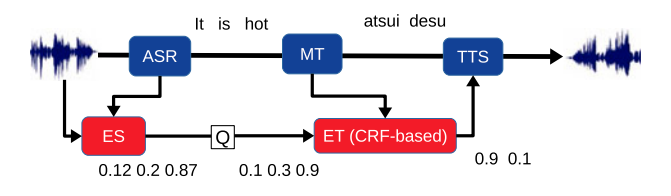
\includegraphics[width=0.7\linewidth]{img/quoc_a.png} \\
(a) CRF-based \\[6pt]
 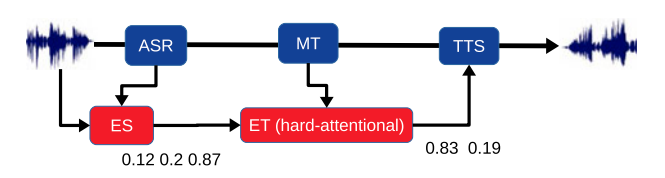
\includegraphics[width=0.7\linewidth]{img/quoc_b.png} \\
(b) Hard-attentional \\[6pt]
 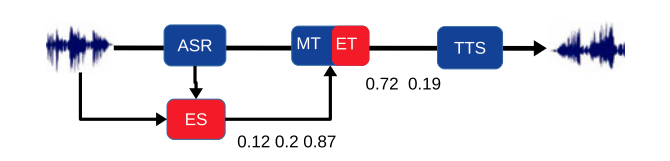
\includegraphics[width=0.7\linewidth]{img/quoc_c.png} \\
(c) Joint model \\[6pt]
\end{tabular}
\caption{Various implementations of S2S translation systems with emphasis transfer. (Diagrams are taken from \cite{Quoc2018}) }
\label{sota:quoc}
\end{figure}

%pause transfer
Pausing in speech is an important prosodic feature that affects both emphasis perception and phrasing. Transfer of pauses within S2S translation is addressed in the works: \cite{truong2015_iwslt} and \cite{bonafonte:pausetransfer}. In the former one, pause prediction is incorporated into the CRF-based emphasis prediction module and shows improvement in terms of emphasis perception in the synthesized examples. The latter work focuses on the transfer of the phrasing and follows a rule-based approach exploiting alignment information from SMT. 

%context enrichment
Some work on use of prosody in S2S translation focuses on employing prosodic features available through acoustic or linguistic analysis to further boost translation accuracy. These works are mostly inspired from approaches where factored SMT is enhanced with linguistic features (e.g.~POS features) and employ a similar approach in spoken translation. \cite{Guo2016} is an example where additional prosodic features based on pronunciation, boundary marks and emphasis is integrated as factors to a factored translation model based system. They record slight improvement in terms of translation accuracy with inclusion of boundary marks when translated from Chinese to English. In the opposite direction, they record improvement with inclusion of all three features. Again in \cite{RangarajanSridhar:2013:enrichingS2S}, factored translation models used for phrase-based translation is extended to accept additional prosodic information on source and target sides. They test inclusion of dialog information such as question types in source side and pitch accent based prominence features on the target side. Modest improvements are recorded in terms of translation accuracy. 